\documentclass[12pt, a4paper]{article}

\usepackage{enumerate}
\usepackage[margin=5em]{geometry}
\usepackage{tikz}
\usetikzlibrary{positioning}
\usetikzlibrary{shapes}

\setlength\parskip{1em}
\setlength\parindent{0em}

\title{Assignment 6}

\author{Hendrik Werner s4549775}

\begin{document}
\maketitle

\section{} %1
\begin{enumerate}[a]
	\item %a
	\item %b
\end{enumerate}

\section{} %2
\begin{enumerate}[a]
	\item %a
	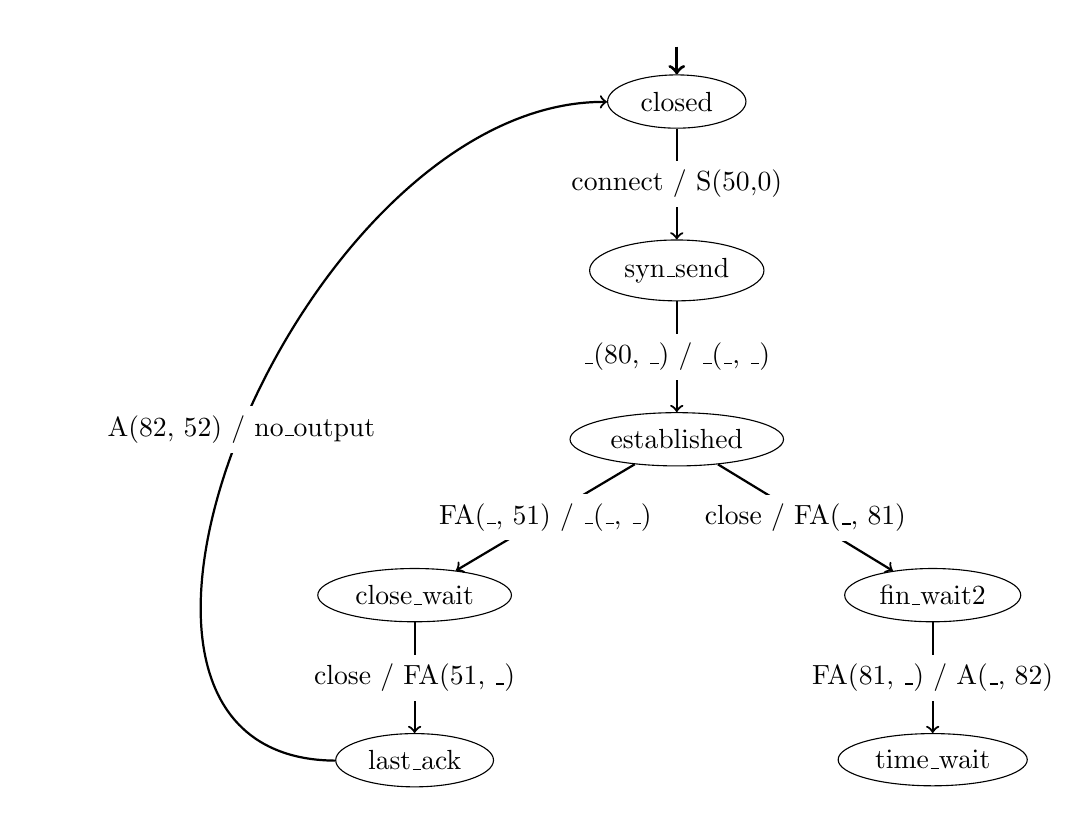
\begin{tikzpicture}[
		node distance=4em,
		n/.style={draw, ellipse, minimum width=5em},
		a/.style={->, thick},
	]
		\node (Start) {};
		\node[n, below=1em of Start] (A) {closed};
		\node[n, below=of A] (B) {syn\_send};
		\node[n, below=of B] (C) {established};
		\node[n, below left=6em of C] (D) {close\_wait};
		\node[n, below right=6em of C] (E) {fin\_wait2};
		\node[n, below=of D] (F) {last\_ack};
		\node[n, below=of E] (G) {time\_wait};

		\draw[a, very thick] (Start) edge (A);
		\draw[a] (A) edge node[fill=white] {connect / S(50,0)} (B);
		\draw[a] (B) edge node[fill=white] {\_(80, \_) / \_(\_, \_)} (C);
		\draw[a] (C) edge node[fill=white] {FA(\_, 51) / \_(\_, \_)} (D);
		\draw[a] (C) edge node[fill=white] {close / FA(\_, 81)} (E);
		\draw[a] (D) edge node[fill=white] {close / FA(51, \_)} (F);
		\draw[a] (E) edge node[fill=white] {FA(81, \_) / A(\_, 82)} (G);
		\draw[a] (F) edge[bend left, out=112, in=112, looseness=1.1] node[fill=white] {A(82, 52) / no\_output} (A);
	\end{tikzpicture}
	\item %b
	\item %c
	\item %d
\end{enumerate}

\section{} %3
\begin{enumerate}[a]
	\item %a
	This is TCP Tahoe because at 14 a new slow start phase is started. Reno would skip this phase.
	\item %b
	The slow start is operating from 1-4 and from 14. It can be identified by the exponential speed increase.
	\item %c
	In the congestion avoidance phase the $cwnd$ (congestion window) is linearly increasing. This happens between 4-8 and 9-13.
	\item %d
	On slide 48 is says that if you are in congestion avoidance mode (which we are at 13) and you receive 3 duplicate ACKs then you go into fast recovery mode. Because at 14 the slow start begins again we can assume that at 13 a timeout happened.
	\item %e
	The $ssthresh$ is initially set to 8 because that it when the slow start phase ends.
	\item %f
	The $ssthresh$ at 8 should be set to half of what it is, so to 6. If you look at the graph however the $ssthresh$ seems to be set to 9 instead because that is where fast recovery picks up.
	\item %g
	The $ssthresh$ is set to half the current $cwnd$ after 13, which is $6$. Because at 15 the $cwnd$ is at 2 and $2^2 = 4 \leq 6$, the $cwnd$ at 16 is 4.
	\item %h
	Both values are set to half the current $cwnd$, which is 1. The $ssthresh$ and $cwnd$ would both be set to 1.
	\item %i
	\begin{tabular}{c|c|c}
		Round & Packets send & Total\\\hline
		1 & 1 & 1\\
		2 & 2 & 3\\
		3 & 4 & 7\\
		4 & 8 & 15\\
		5 & 9 & 24\\
	\end{tabular}

	The 17th segment is send somewhere within the 5th round.
\end{enumerate}

\end{document}
